
% Copyright (c)  2007-2012  Tim Niemueller, RWTH Aachen University
%
% Created: Mon Aug 13 16:55:22 2012

%aspectratio=169
\documentclass[compress,xcolor=table,nominiframes,notitlehead,noframetitlebg,addurl]{beamer}
% add handout to optional args for handout version

%\usepackage{hyperref}
\usepackage{beamerthemesplit}
\usepackage[utf8]{inputenc}
\usepackage[T1]{fontenc}
\usepackage[german]{babel}
\usepackage{german}
\usepackage{graphicx}
\usepackage{subfigure}
\usepackage{epsfig}
\usepackage{tabularx}
\usepackage{latexsym}
\usepackage{url}
\usepackage{tikz}
\usepackage{multimedia}
\usepackage{xcolor}
\usepackage{listings}
\usepackage{verbatim}
\usepackage{colortbl}
\usepackage{psfrag}
\usepackage{xifthen}
\usepackage[absolute,overlay]{textpos}
\usepackage{palatino}
\usepackage{enumitem}

\graphicspath{{../},{./images/},{./images/},{./figures/}}

%% Mulberry Color for highlighting
\definecolor{Mulberry}{cmyk}{0.34,0.90,0,0.02}
\definecolor{Lavender}{cmyk}{0,0.48,0,0}
\definecolor{Melon}{cmyk}{0,0.46,0.50,0}
\definecolor{Peach}{cmyk}{0,0.50,0.70,0}
\definecolor{RedOrange}{cmyk}{0,0.77,0.87,0}
\definecolor{BrickRed}{cmyk}{0,0.89,0.94,0.28}
\definecolor{Mahogany}{cmyk}{0,0.85,0.87,0.35}
\definecolor{BurntOrange}{cmyk}{0,0.51,1,0}
\definecolor{BitterSweet}{cmyk}{0,0.75,1,0.24}
\definecolor{RosBlue}{rgb}{0.19,0.25,0.38}


\mode<presentation>
{
  \usetheme{FawkesMinimal}

  % to hide nav bar uncomment this line
  \setbeamertemplate{navigation symbols}{}

  %\setbeamercovered{transparent}
  \setbeamercovered{%
    invisible,
    again covered={\opaqueness<1->{40}}
  }

  \setbeamerfont{author}{size=\footnotesize,family=\rmfamily,parent=structure}
}

% Usage notes for handout version:
% Compile the beamer version immediately before you build the handout version,
% otherwise page numbers etc. will be wrong! The .aux files are *not* updated
% in handout mode, see PGF Manual for details why this is necessary.
% Comment out below one of the two pgfuselayout lines for either 2 or 4 slides
% per page. To have a very light grey background uncomment the background canvas
% color line. The logical page options are used to draw borders around each
% slide.
\mode<handout>
{
  \usetheme{Fawkes}

  % to hide nav bar uncomment this line
  \setbeamertemplate{navigation symbols}{}

  %\setbeamercovered{transparent}
  \setbeamercovered{%
    again covered={\opaqueness<1->{40}}
  }

  % Very slight grey background, can be used instead of borders
  %\setbeamercolor{background canvas}{bg=black!5}

  \usepackage{pgfpages}
  \pgfpagesuselayout{4 on 1}[a4paper,border shrink=5mm,landscape]
  %\pgfpagesuselayout{2 on 1}[a4paper,border shrink=5mm]

  \pgfpageslogicalpageoptions{1}{border code=\pgfstroke}
  \pgfpageslogicalpageoptions{2}{border code=\pgfstroke}
  \pgfpageslogicalpageoptions{3}{border code=\pgfstroke}
  \pgfpageslogicalpageoptions{4}{border code=\pgfstroke}
  \nofiles
}


% Declare layers
\pgfdeclarelayer{background}
\pgfsetlayers{background,main} 

% Load PGF libraries
\usetikzlibrary{patterns}
\usetikzlibrary{arrows}
\usetikzlibrary{topaths}
\usetikzlibrary{snakes}
\usetikzlibrary{calc}
\usetikzlibrary{positioning}
\usetikzlibrary{shadows}
\usetikzlibrary{shapes.multipart}
\usetikzlibrary{arrows.meta}
\usetikzlibrary{fit,arrows,decorations.pathreplacing,decorations.text}


% set lengths for textpos package
\setlength{\TPHorizModule}{10mm}
\setlength{\TPVertModule}{\TPHorizModule}
\textblockorigin{8mm}{16mm} % start everything near the top-left corner
\setbeamercolor{textblock color}{fg=blue!50,bg=white}

\institute{%
  %\vspace{1cm}
  \begin{minipage}{\textwidth}\centering
  
\includegraphics[height=0.6cm]{common/images/logos/rwth-logo}
  \quad\quad
  
\includegraphics[height=0.6cm]{common/images/logos/kbsg}
  \end{minipage}
}

\setlist[itemize]{leftmargin=12pt,label=\usebeamerfont*{itemize item}%
  \usebeamercolor[fg]{itemize item}
  \usebeamertemplate{itemize item}}
\setlist[description]{leftmargin=4pt,itemindent=0pt,font=\color{FawkesOrange}}
\setenumerate[1]{%
  leftmargin=12pt,%
  label=\protect\usebeamerfont{enumerate item}%
        \protect\usebeamercolor[fg]{enumerate item}%
        \insertenumlabel.}

%numbers=left, numberstyle=\tiny, stepnumber=2, numbersep=5pt
\lstset{language=[GNU]C++,
        basicstyle=\small,
        escapeinside={/*(*/}{/*)*/},
        breaklines=true,
        showstringspaces=false
        }

% Uncomment the listings styles you need
\lstdefinelanguage{Lua}
{
  morekeywords={and,break,do,else,elseif,end,false,for,function,
                if,in,local,nil,not,or,repeat,return,then,true,until,while},
  sensitive=true,
  morecomment=[l]{--},
  morecomment=[s]{--[[}{--]]},
  morestring=[b]{"},
  morestring=[s]{[==[}{]==]},
}

% default style
\lstdefinestyle{Lua}
{
  language=Lua,
  basicstyle=\ttfamily,
  breaklines=true,
  showstringspaces=false,
  %keywordstyle=\bfseries,
  keywordstyle=\color{Mulberry},
  %frame=lines,
  %belowcaptionskip=8pt,
  emphstyle=\itshape,
  %numbers=left,
  stepnumber=1,
  %backgroundcolor=\color{blue!10},
  rulecolor=\color{blue!50},
  fillcolor=\color{blue!20},
  %framexleftmargin=18pt,
  %xleftmargin=18pt,
  stringstyle=\color{BitterSweet},
  %stringstyle=\color{BrickRed},
  commentstyle=\color{BrickRed},
  escapechar=\%
  % emph={getup, servo, depends_skills},
  %emphstyle=\underbar,
  %numbers=left,
  %stepnumber=1,
  %%stringstyle=\ttfamily, % typewriter type for strings
}
\lstdefinestyle{SmallLua}{
  style=Lua,
  basicstyle=\ttfamily\footnotesize,
  numbersep=6pt,
}
\lstdefinestyle{ReallySmallLua}{
  style=Lua,
  basicstyle=\ttfamily\tiny,
  numbersep=5pt,
}

\lstdefinelanguage{Yaml}
{
  keywords={true,false,null,y,n},
  sensitive=false,
  comment=[l]{\#},
  morecomment=[s]{/*}{*/},
  morestring=[b]',
  morestring=[b]",
}

% default style
\lstdefinestyle{Yaml}
{
  language=Yaml,
  basicstyle=\YAMLkeystyle,
  breaklines=true,
  showstringspaces=false,
  %keywordstyle=\bfseries,
  keywordstyle=\color{Mulberry},
  %frame=lines,
  %belowcaptionskip=8pt,
  emphstyle=\itshape,
  %numbers=left,
  stepnumber=1,
  %backgroundcolor=\color{blue!10},
  rulecolor=\color{blue!50},
  fillcolor=\color{blue!20},
  %framexleftmargin=18pt,
  %xleftmargin=18pt,
  stringstyle=\color{BitterSweet},
  %stringstyle=\color{BrickRed},
  commentstyle=\color{BrickRed},
  escapechar=\%
  % emph={getup, servo, depends_skills},
  %emphstyle=\underbar,
  %numbers=left,
  %stepnumber=1,
  %%stringstyle=\ttfamily, % typewriter type for strings
}
\lstdefinestyle{SmallYaml}{
  style=Yaml,
  basicstyle=\ttfamily\footnotesize,
  numbersep=6pt,
}
\lstdefinestyle{ReallySmallYaml}{
  style=Yaml,
  basicstyle=\ttfamily\tiny,
  numbersep=5pt,
}

%\lstdefinelanguage{OpenPRS}{
  keywordsprefix=\$,
  %keywordsprefix=\$,
  alsoletter={?!=-<>*\$^~},
  keywordstyle=\color{Mulberry!80!black}\bfseries,
  keywords=[2]{:invocation, :context, :call, :body, :action,
    :setting, :documentation, :effects, defop},
  keywordstyle=[2]\color{BrickRed!70!blue}\bfseries,
  keywords=[3]{?, !, ^, ~, =>, ~>, =, if, else, elseif, do, while, //},
  keywordstyle=[3]\color{darkgray}\bfseries,
  keywords=[4]{start-critical-section, end-critical-section, equal,
    print, printf},%
  keywordstyle=[4]\color{gray}\bfseries,
  %identifierstyle=\color{black},
  sensitive=false,
  comment=[l]{;},
  commentstyle=\color{purple}\ttfamily,
  stringstyle=\color{red}\ttfamily,
  morestring=[b]"
}


\lstdefinestyle{OpenPRS}
{
  language=OpenPRS,
  basicstyle=\footnotesize\ttfamily\vspace{0.2cm},
  breaklines=true,
  showstringspaces=false,
  %keywordstyle=\bfseries,
  %keywordstyle=\color{Mulberry},
  frame=lines,
  belowcaptionskip=8pt,
  emphstyle=\itshape,
  numbers=left,
  stepnumber=1,
  backgroundcolor=\color{blue!10},
  rulecolor=\color{blue!50},
  fillcolor=\color{blue!20},
  framexleftmargin=16pt,
  xleftmargin=16pt,
  %stringstyle=\color{BitterSweet},
  stringstyle=\color{BrickRed},
  commentstyle=\color{BrickRed},
  escapechar=\%
  % emph={getup, servo, depends_skills},
  %emphstyle=\underbar,
  %numbers=left,
  %stepnumber=1,
  %%stringstyle=\ttfamily, % typewriter type for strings
}

\lstdefinestyle{SmallOpenPRS}{
  style=OpenPRS,
  basicstyle=\ttfamily\footnotesize,
  numbersep=6pt,
}
\lstdefinestyle{ReallySmallOpenPRS}{
  style=OpenPRS,
  basicstyle=\ttfamily\scriptsize,
  numbersep=5pt,
}

\lstdefinestyle{ReallySmallOpenPRSNoFrame}{
  style=OpenPRS,
  basicstyle=\ttfamily\scriptsize,
  numbersep=5pt,
  frame=none,
  backgroundcolor=\color{white},
  framextopmargin=0pt,
  framexbottommargin=0pt
}

\lstdefinestyle{SuperSmallOpenPRSNoFrame}{
  style=OpenPRS,
  basicstyle=\ttfamily\fontsize{10pt}{10pt}\selectfont,
  numbers=none,
  frame=none,
  backgroundcolor=\color{white},
  framextopmargin=0pt,
  framexbottommargin=0pt,
  framexleftmargin=-2pt, xleftmargin=-2pt,
}

\lstdefinestyle{SmallOpenPRSNoFrame}{
  style=OpenPRS,
  basicstyle=\ttfamily\footnotesize,
  numbersep=5pt,
  frame=none,
  backgroundcolor=\color{white},
  framextopmargin=0pt,
  framexbottommargin=0pt
}

\lstdefinelanguage{CLIPS}{
  keywordsprefix=?,
  %keywordsprefix=\$,
  alsoletter={?=-<>*\$},
  keywordstyle=\color{Mulberry!80!black}\bfseries,
  keywords=[2]{deffunction, deftemplate, defrule, deffacts, defgeneric,
    defmodule, defadvice, defglobal, defmethod, definstance, defclass},
  keywordstyle=[2]\color{BrickRed!70!blue}\bfseries,
  keywords=[3]{slot, multislot, type, default, default-dynamic,
                      extends, crlf, range, nil, if, then, else, while,
                      not, or, switch, case, and, reset,
                      assert, test, declare, salience, return, bind, modify,
                      retract, explicit, unique, node-index-hash,
                      halt, printout, =>, <-},
  keywordstyle=[3]\color{darkgray}\bfseries,
  keywords=[4]{subsetp,progn, progn$, not, node-index-hash, create$,
    append$, length$, printout},%
  keywordstyle=[4]\color{gray}\bfseries,
  %identifierstyle=\color{black},
  sensitive=false,
  comment=[l]{;},
  commentstyle=\color{purple}\ttfamily,
  stringstyle=\color{red}\ttfamily,
  morestring=[b]"
}


\lstdefinestyle{CLIPS}
{
  language=CLIPS,
  basicstyle=\footnotesize\ttfamily\vspace{0.2cm},
  breaklines=true,
  showstringspaces=false,
  %keywordstyle=\bfseries,
  %keywordstyle=\color{Mulberry},
  frame=lines,
  belowcaptionskip=-3pt,
  emphstyle=\itshape,
  numbers=left,
  stepnumber=1,
  backgroundcolor=\color{gray!10},
  rulecolor=\color{gray!80},
  fillcolor=\color{gray!10},
  framexleftmargin=16pt,
  xleftmargin=16pt,
  %stringstyle=\color{BitterSweet},
  stringstyle=\color{BrickRed},
  commentstyle=\color{BrickRed},
  escapechar=\%,
  % emph={getup, servo, depends_skills},
  %emphstyle=\underbar,
  %numbers=left,
  %stepnumber=1,
  %%stringstyle=\ttfamily, % typewriter type for strings
  %float,
  captionpos=b
}

\lstdefinestyle{SmallCLIPS}{
  style=CLIPS,
  basicstyle=\ttfamily\footnotesize,
  numbersep=6pt,
}
\lstdefinestyle{ReallySmallCLIPS}{
  style=CLIPS,
  basicstyle=\ttfamily\scriptsize,
  numbersep=5pt,
}

\lstdefinestyle{ReallySmallCLIPSNoFrame}{
  style=CLIPS,
  basicstyle=\ttfamily\scriptsize,
  numbersep=5pt,
  frame=none,
  backgroundcolor=\color{white},
  framextopmargin=0pt,
  framexbottommargin=0pt
}

\lstdefinestyle{SuperSmallCLIPSNoFrame}{
  style=CLIPS,
  basicstyle=\ttfamily\fontsize{10pt}{10pt}\selectfont,
  numbers=none,
  frame=none,
  backgroundcolor=\color{white},
  framextopmargin=0pt,
  framexbottommargin=0pt,
  framexleftmargin=-2pt, xleftmargin=-2pt,
}

\lstdefinestyle{SmallCLIPSNoFrame}{
  style=CLIPS,
  basicstyle=\ttfamily\footnotesize,
  numbersep=5pt,
  frame=none,
  backgroundcolor=\color{white},
  framextopmargin=0pt,
  framexbottommargin=0pt
}

%\lstdefinelanguage{JavaScript}{
  keywords={typeof, new, true, false, catch, function, return, null, catch, switch, var, if, in, while, do, else, case, break},
  keywordstyle=\color{blue}\bfseries,
  ndkeywords={class, export, boolean, throw, implements, import}, %, this
  ndkeywordstyle=\color{darkgray}\bfseries,
  identifierstyle=\color{black},
  sensitive=false,
  comment=[l]{//},
  morecomment=[s]{/*}{*/},
  commentstyle=\color{purple}\ttfamily,
  stringstyle=\color{red}\ttfamily,
  morestring=[b]',
  morestring=[b]"
}

\lstdefinestyle{JSON}
{
  language=JavaScript,
  morekeywords={interface,field,message,comment},
  basicstyle=\footnotesize\ttfamily\vspace{0.2cm},
  breaklines=true,
  showstringspaces=false,
  %keywordstyle=\bfseries,
  keywordstyle=\color{Mulberry},
  frame=lines,
  belowcaptionskip=8pt,
  emphstyle=\itshape,
  numbers=left,
  stepnumber=1,
  backgroundcolor=\color{blue!10},
  rulecolor=\color{blue!50},
  fillcolor=\color{blue!20},
  framexleftmargin=16pt,
  xleftmargin=16pt,
  %stringstyle=\color{BitterSweet},
  stringstyle=\color{BrickRed},
  commentstyle=\color{BrickRed},
  escapechar=\%,
  % emph={getup, servo, depends_skills},
  %emphstyle=\underbar,
  %numbers=left,
  %stepnumber=1,
  %%stringstyle=\ttfamily, % typewriter type for strings
  captionpos=b
}

\lstdefinestyle{SmallJSON}{
  style=JSON,
  basicstyle=\ttfamily\footnotesize,
  numbersep=6pt,
}
\lstdefinestyle{ReallySmallJSON}{
  style=JSON,
  basicstyle=\ttfamily\tiny,
  numbersep=5pt,
}

\definecolor{dkgreen}{rgb}{0,0.6,0}
\definecolor{gray}{rgb}{0.5,0.5,0.5}
\definecolor{mauve}{rgb}{0.58,0,0.82}
\definecolor{gray}{rgb}{0.4,0.4,0.4}
\definecolor{darkblue}{rgb}{0.0,0.0,0.6}
\definecolor{lightblue}{rgb}{0.0,0.0,0.9}
\definecolor{cyan}{rgb}{0.0,0.6,0.6}
\definecolor{darkred}{rgb}{0.6,0.0,0.0}


\lstdefinelanguage{XML}
{
  basicstyle=\ttfamily\footnotesize,
  columns=fullflexible,
  showstringspaces=false,
  numbers=left,                   % where to put the line-numbers
  numberstyle=\tiny\color{gray},  % the style that is used for the line-numbers
  stepnumber=1,
  numbersep=5pt,                  % how far the line-numbers are from the code
  backgroundcolor=\color{white},      % choose the background color. You must add \usepackage{color}
  showspaces=false,               % show spaces adding particular underscores
  showstringspaces=false,         % underline spaces within strings
  showtabs=false,                 % show tabs within strings adding particular underscores
  frame=none,                   % adds a frame around the code
  rulecolor=\color{black},        % if not set, the frame-color may be changed on line-breaks within not-black text (e.g. commens (green here))
  tabsize=2,                      % sets default tabsize to 2 spaces
  captionpos=b,                   % sets the caption-position to bottom
  breaklines=true,                % sets automatic line breaking
  breakatwhitespace=false,        % sets if automatic breaks should only happen at whitespace
  title=\lstname,                   % show the filename of files included with \lstinputlisting;
                                  % also try caption instead of title  
  commentstyle=\color{gray}\upshape,
  morestring=[s][\color{mauve}]{"}{"},
  morestring=[s][\color{black}]{>}{<},
  morecomment=[s]{<?}{?>},
  morecomment=[s][\color{dkgreen}]{<!--}{-->},
  stringstyle=\color{black},
  identifierstyle=\color{lightblue},
  keywordstyle=\color{red},
  morekeywords={xmlns,xsi,noNamespaceSchemaLocation,type,id,x,y,source,target,version,tool,transRef,roleRef,objective,eventually},
  basicstyle=\ttfamily\scriptsize,
  backgroundcolor=\color{blue!10},
  numbers=none,
  numbersep=5pt
}


% Default style
\lstset{style=Lua}

% Hyphenation of words with hyphen
\def\hyph{-\penalty0\hskip0pt\relax}

% define an anchor in the frame
\newcommand{\tikzref}[1]{%
  \tikz[remember picture]{%
    \coordinate (#1) at (0,0.5ex);%
  }%
}%


%%% Local Variables: 
%%% mode: latex
%%% TeX-master: "aaai-spring2013-clips-agent"
%%% End: 

\lstdefinelanguage{CLIPS}{
  keywordsprefix=?,
  %keywordsprefix=\$,
  alsoletter={?=-<>*\$},
  keywordstyle=\color{Mulberry!80!black}\bfseries,
  keywords=[2]{deffunction, deftemplate, defrule, deffacts, defgeneric,
    defmodule, defadvice, defglobal, defmethod, definstance, defclass},
  keywordstyle=[2]\color{BrickRed!70!blue}\bfseries,
  keywords=[3]{slot, multislot, type, default, default-dynamic,
                      extends, crlf, range, nil, if, then, else, while,
                      not, or, switch, case, and, reset,
                      assert, test, declare, salience, return, bind, modify,
                      retract, explicit, unique, node-index-hash,
                      halt, printout, =>, <-},
  keywordstyle=[3]\color{darkgray}\bfseries,
  keywords=[4]{subsetp,progn, progn$, not, node-index-hash, create$,
    append$, length$, printout},%
  keywordstyle=[4]\color{gray}\bfseries,
  %identifierstyle=\color{black},
  sensitive=false,
  comment=[l]{;},
  commentstyle=\color{purple}\ttfamily,
  stringstyle=\color{red}\ttfamily,
  morestring=[b]"
}


\lstdefinestyle{CLIPS}
{
  language=CLIPS,
  basicstyle=\footnotesize\ttfamily\vspace{0.2cm},
  breaklines=true,
  showstringspaces=false,
  %keywordstyle=\bfseries,
  %keywordstyle=\color{Mulberry},
  frame=lines,
  belowcaptionskip=-3pt,
  emphstyle=\itshape,
  numbers=left,
  stepnumber=1,
  backgroundcolor=\color{gray!10},
  rulecolor=\color{gray!80},
  fillcolor=\color{gray!10},
  framexleftmargin=16pt,
  xleftmargin=16pt,
  %stringstyle=\color{BitterSweet},
  stringstyle=\color{BrickRed},
  commentstyle=\color{BrickRed},
  escapechar=\%,
  % emph={getup, servo, depends_skills},
  %emphstyle=\underbar,
  %numbers=left,
  %stepnumber=1,
  %%stringstyle=\ttfamily, % typewriter type for strings
  %float,
  captionpos=b
}

\lstdefinestyle{SmallCLIPS}{
  style=CLIPS,
  basicstyle=\ttfamily\footnotesize,
  numbersep=6pt,
}
\lstdefinestyle{ReallySmallCLIPS}{
  style=CLIPS,
  basicstyle=\ttfamily\scriptsize,
  numbersep=5pt,
}

\lstdefinestyle{ReallySmallCLIPSNoFrame}{
  style=CLIPS,
  basicstyle=\ttfamily\scriptsize,
  numbersep=5pt,
  frame=none,
  backgroundcolor=\color{white},
  framextopmargin=0pt,
  framexbottommargin=0pt
}

\lstdefinestyle{SuperSmallCLIPSNoFrame}{
  style=CLIPS,
  basicstyle=\ttfamily\fontsize{10pt}{10pt}\selectfont,
  numbers=none,
  frame=none,
  backgroundcolor=\color{white},
  framextopmargin=0pt,
  framexbottommargin=0pt,
  framexleftmargin=-2pt, xleftmargin=-2pt,
}

\lstdefinestyle{SmallCLIPSNoFrame}{
  style=CLIPS,
  basicstyle=\ttfamily\footnotesize,
  numbersep=5pt,
  frame=none,
  backgroundcolor=\color{white},
  framextopmargin=0pt,
  framexbottommargin=0pt
}

\lstdefinelanguage{JavaScript}{
  keywords={typeof, new, true, false, catch, function, return, null, catch, switch, var, if, in, while, do, else, case, break},
  keywordstyle=\color{blue}\bfseries,
  ndkeywords={class, export, boolean, throw, implements, import}, %, this
  ndkeywordstyle=\color{darkgray}\bfseries,
  identifierstyle=\color{black},
  sensitive=false,
  comment=[l]{//},
  morecomment=[s]{/*}{*/},
  commentstyle=\color{purple}\ttfamily,
  stringstyle=\color{red}\ttfamily,
  morestring=[b]',
  morestring=[b]"
}

\lstdefinestyle{JSON}
{
  language=JavaScript,
  morekeywords={interface,field,message,comment},
  basicstyle=\footnotesize\ttfamily\vspace{0.2cm},
  breaklines=true,
  showstringspaces=false,
  %keywordstyle=\bfseries,
  keywordstyle=\color{Mulberry},
  frame=lines,
  belowcaptionskip=8pt,
  emphstyle=\itshape,
  numbers=left,
  stepnumber=1,
  backgroundcolor=\color{blue!10},
  rulecolor=\color{blue!50},
  fillcolor=\color{blue!20},
  framexleftmargin=16pt,
  xleftmargin=16pt,
  %stringstyle=\color{BitterSweet},
  stringstyle=\color{BrickRed},
  commentstyle=\color{BrickRed},
  escapechar=\%,
  % emph={getup, servo, depends_skills},
  %emphstyle=\underbar,
  %numbers=left,
  %stepnumber=1,
  %%stringstyle=\ttfamily, % typewriter type for strings
  captionpos=b
}

\lstdefinestyle{SmallJSON}{
  style=JSON,
  basicstyle=\ttfamily\footnotesize,
  numbersep=6pt,
}
\lstdefinestyle{ReallySmallJSON}{
  style=JSON,
  basicstyle=\ttfamily\tiny,
  numbersep=5pt,
}


\usepackage{todonotes}
\usepackage{booktabs}
\newcommand{\tabitem}{~~\llap{\textcolor{FawkesOrange}{\textbullet}}~~}

\hypersetup{
  pdftitle      = {RobotMemory-Proposal-Talk},
  pdfauthor     = {Frederik Zwilling},
  pdfkeywords   = {robotics, artificial intelligence, robot memory, logistics, RCLL, @Home},
  pdfsubject    = {Master Thesis Proposal Talk}
  %hidelinks    = true
}

\title[Robot Memory] {A Document-Oriented Robot Memory\\ for
  Knowledge Sharing and Hybrid Reasoning\\ on Mobile Robots}
\author[Zwilling]{
  \textbf{Frederik Zwilling}\\
  ~Adviser: Tim Niemueller\\
  ~Supervisors: Prof. Lakemeyer, PhD., Prof. Dr. Jarke
}
\def\projecturl{}

\date[Aug 16th 2016]{Aug 16th 2016 -- Master Thesis Proposal}

\begin{document}
\shorthandoff{"} % aus "o kein ö machen

\frame[plain]{\titlepage}
\addtocounter{framenumber}{-1}
%% \begin{frame}
%%   \tableofcontents[]
%% \end{frame}
%% \addtocounter{framenumber}{-1}

\section{Motivation}

\begin{frame}
  \frametitle{Motivation}
  \Large{Why do robots need a memory?}
  \vspace{1cm}
  \begin{columns}
    \begin{column}{0.5\textwidth}
    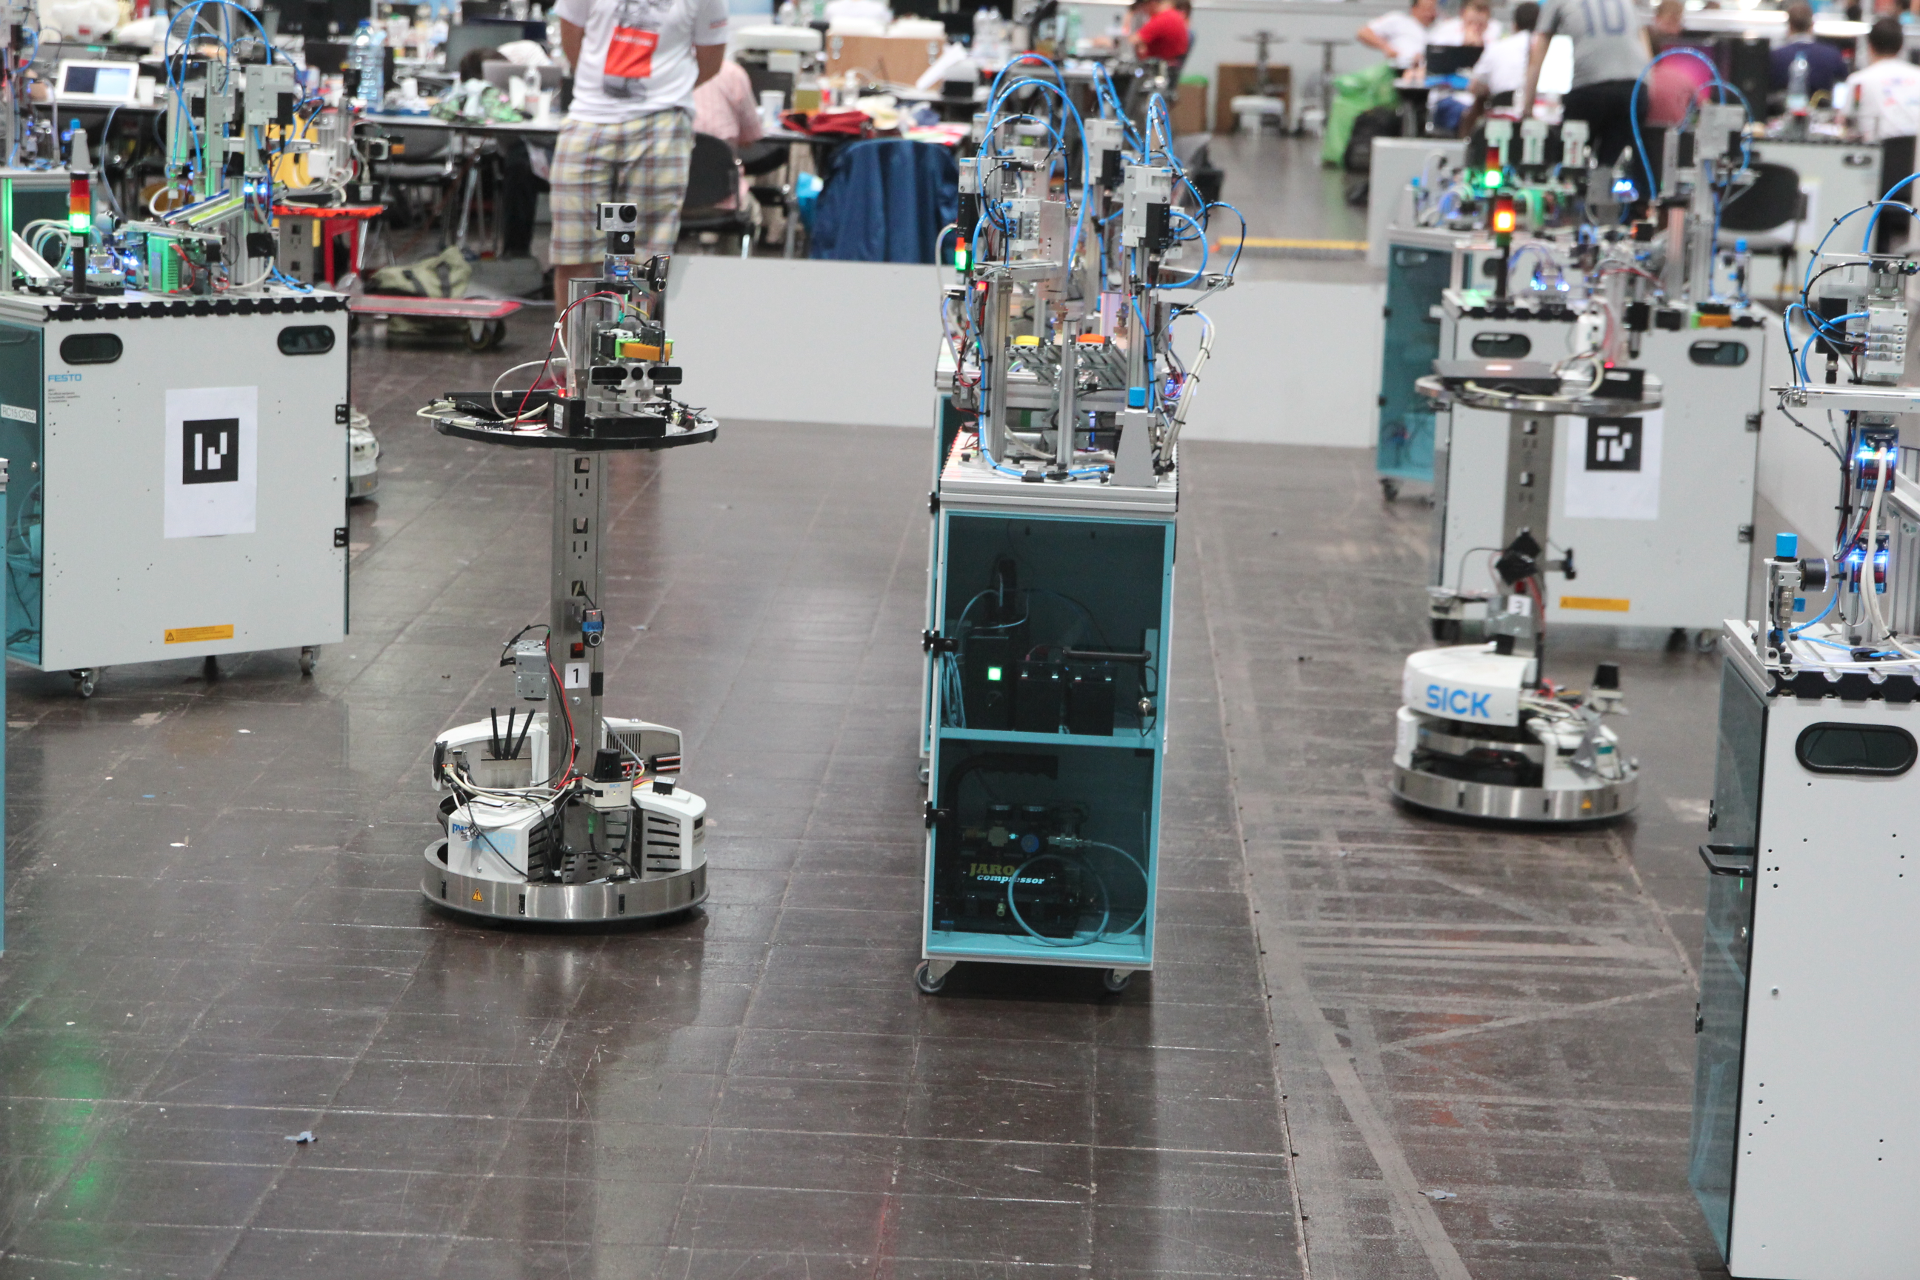
\includegraphics[width=\textwidth]{../img/rcll-feld}
%% Logistics robots in the RCLL (everyone familiar?)
%% need memory to model the state of the world (e.g. product location, orders done)
%% multi-robot locks, tasks being done
%% share knowledge to collaborate
    \end{column}
    \begin{column}{0.5\textwidth}
    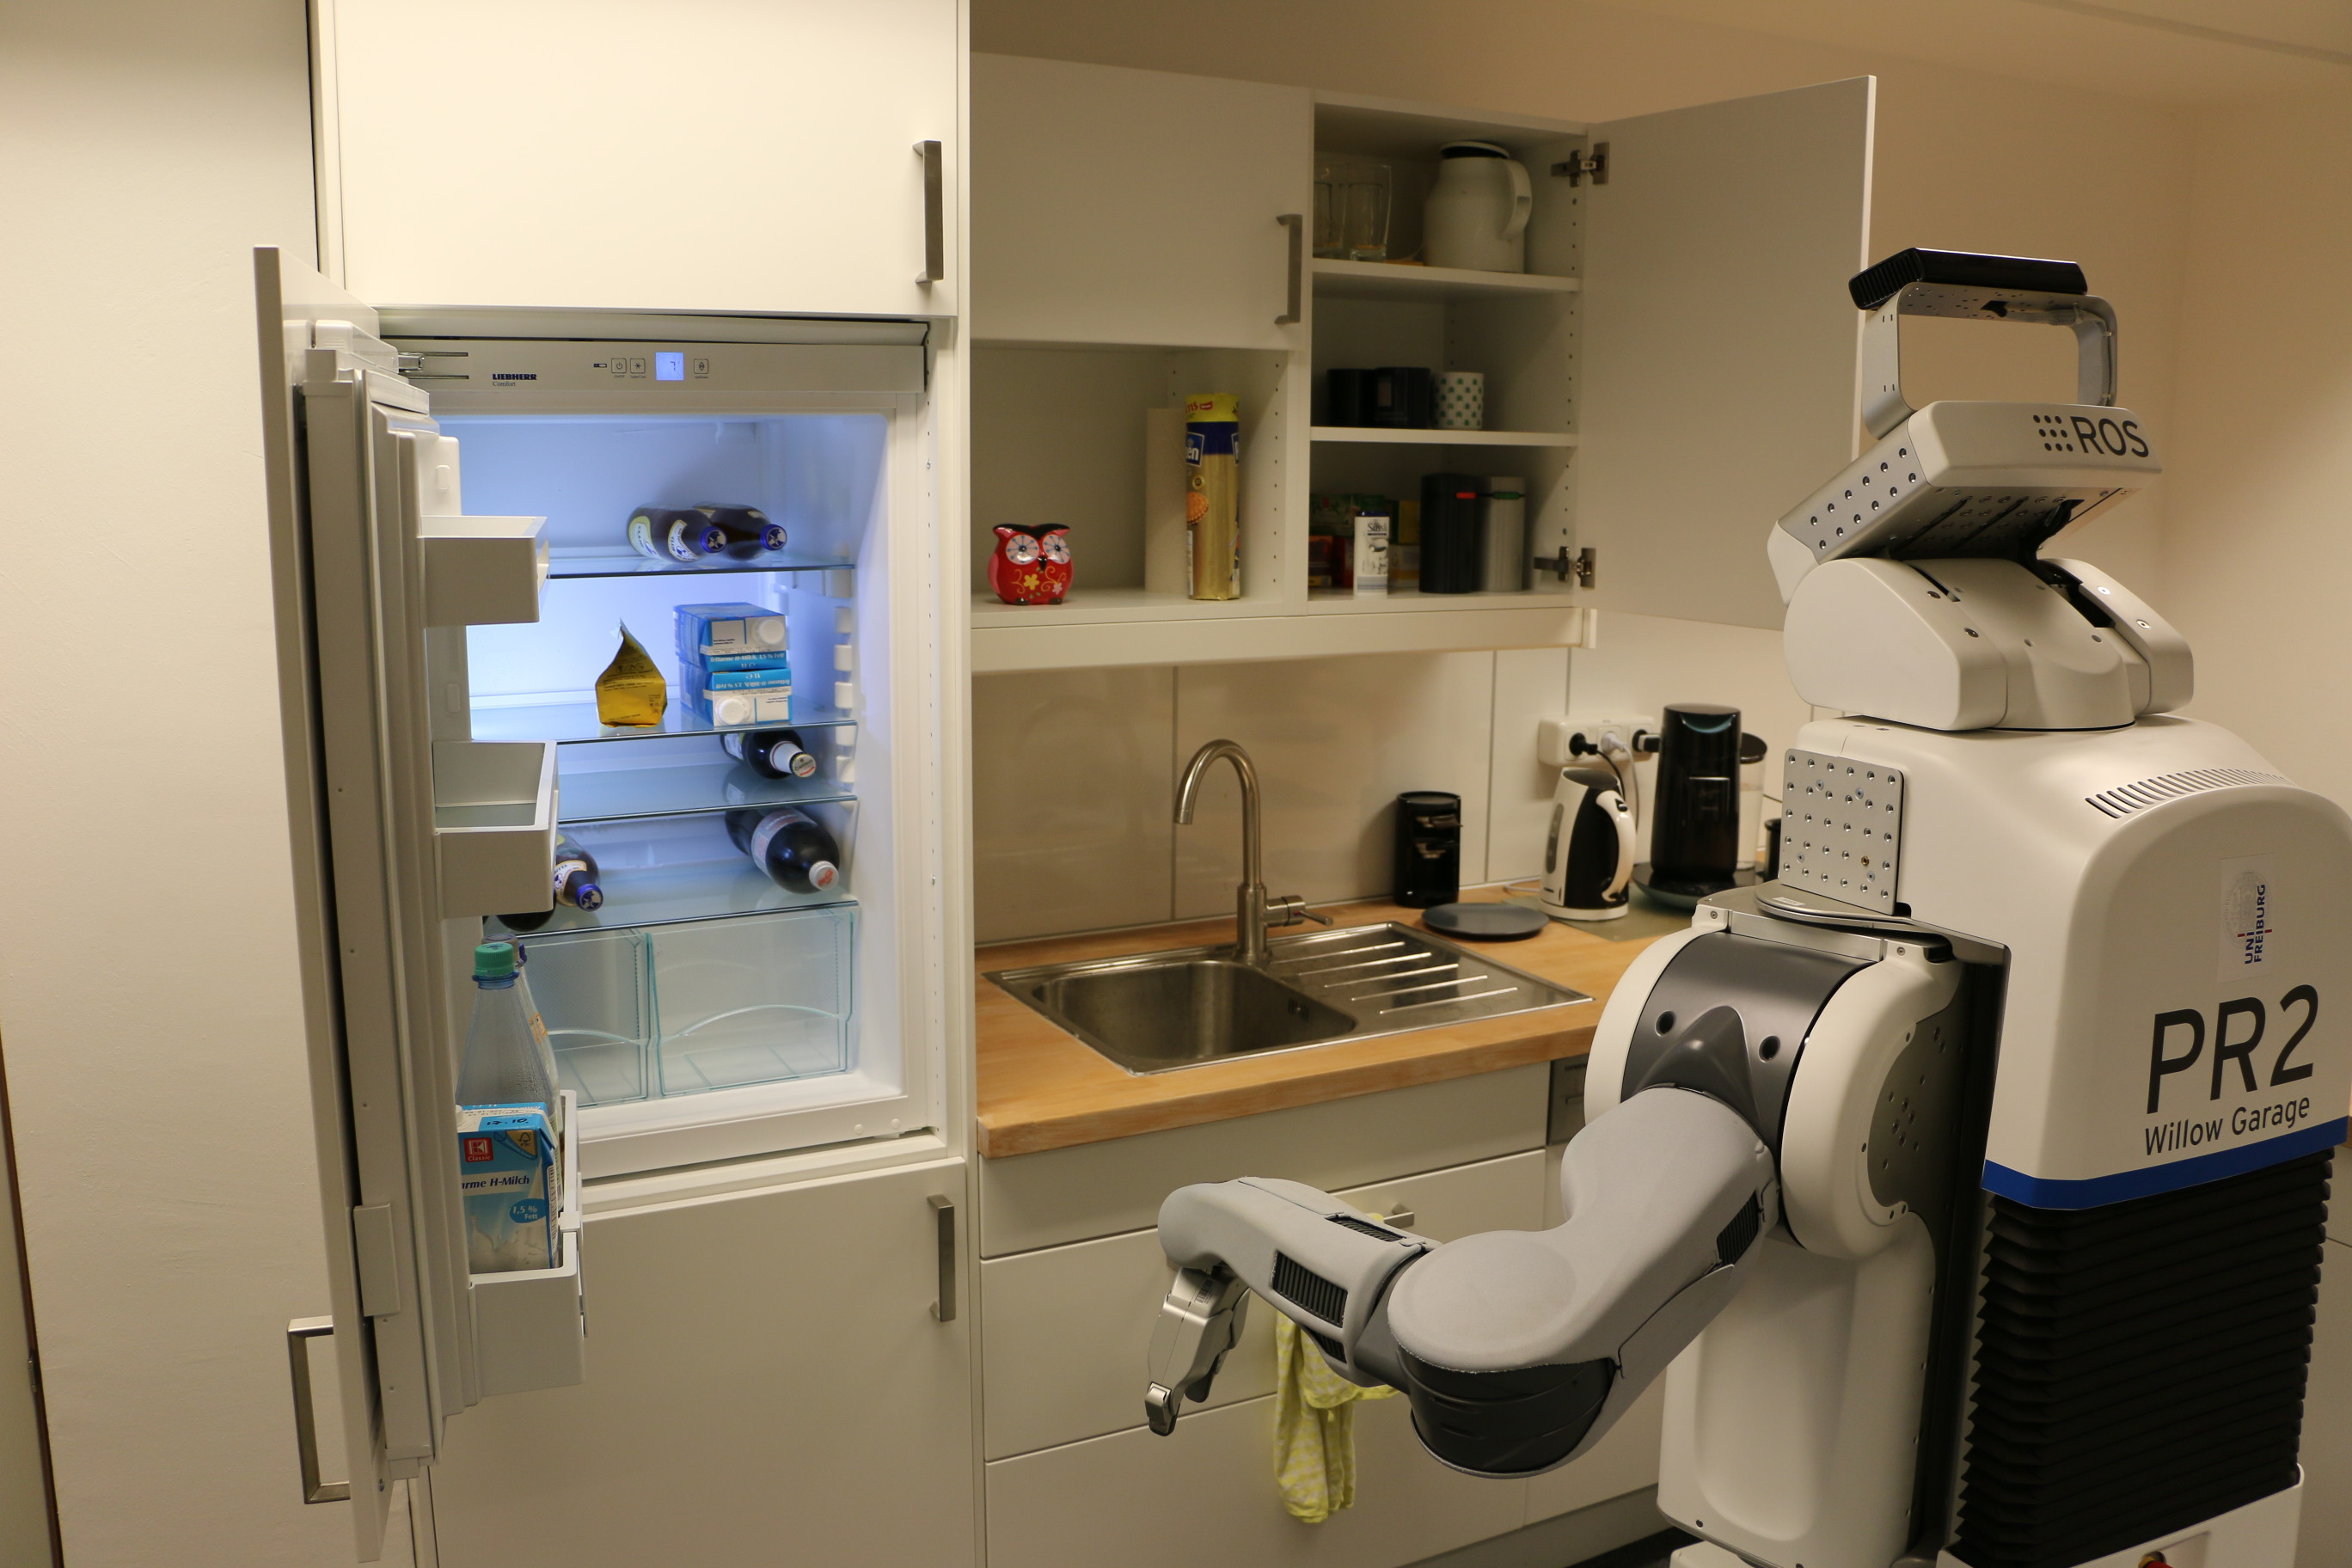
\includegraphics[width=\textwidth]{../img/pr2-kbsg-kitchen}
%% Domestic service robot
%% need memory to model the state of the world (e.g. object locations, user preferences)
%% object sights to derive spatio-temporal distribution (Deebul)
%% persistent storage (rebooting)
    \end{column}
  \end{columns}
\end{frame}

\begin{frame}
  \frametitle{Problem Description - Proposed Solution}
  \begin{columns}
    \begin{column}{0.58\textwidth}
  \begin{description}[]
  \item[Problems of existing approaches]<uncover@1-> \hfill \\
    \begin{itemize}
        \item Static data structure
        \item Memory intertwined in single Knowledge Based System
        \item Locality
        \item Multiple state estimations, inconsistencies
        \item Spatio-Temporal vs. Symbolic
        \item Not scalable, efficient
        \item Not persistent
    \end{itemize}
  \end{description}
    \end{column}
    \begin{column}{0.48\textwidth}
  \begin{description}[]
  \item[Proposed Robot Memory]<uncover@2-> \hfill \\
    \begin{itemize}
        \item Generic representation 
        \item Decoupled Memory from sources and consumers
        \item Distributed for robot teams
        \item Central, consistent storage\\\hfill
        \item On demand computation
        \item Scalable basis
        \item Persistent
    \end{itemize}
  \end{description}
    \end{column}
  \end{columns}
\end{frame}

\section{Related Work}
\begin{frame}
  \frametitle{Related Work: Knowledge Processing Systems}
  \begin{description}[]
  \item[KnowRob/OpenRobots Ontology (ORO)]<uncover@1-> \hfill \\
    \begin{itemize}
    \item Common sense reasoning with ontologies
          %explain with example (graph, rdf, milk)
    \item Virtual knowledge base to interface perception/\\
          Events notifying about changes
    \item Based on Prolog/Java
    \end{itemize}
  \end{description}
  \begin{block}{}<uncover@2->
  \begin{itemize}
  \item Not applicable for multi-robot systems
  \item Scalability, efficiency concerns
  \item Missing events/knowledge computation on demand
  \end{itemize}
  \end{block}
  \begin{description}
  %% \item[OpenRobots Ontology (ORO)]<uncover@1-> \hfill \\
  %%   \begin{itemize}
  %%   \item Focus on human-robot interaction with ontologies
  %%   \item Modular architecture (knowledge decay, categorization)
  %%         %for short time memory, find missing information
  %%   \item Events notifying about changes
  %%   \end{itemize}
  \item[Generic Robot Database with MongoDB]<uncover@3-> \hfill \\
    \begin{itemize}
    \item Data logging for evaluation and fault analysis
    \item Generic and scalable storage with MongoDB
    \item Integration in Fawkes and ROS
    \end{itemize}
  \end{description}
\end{frame}

%% \begin{frame}
%%   \frametitle{Related Work}
%%   \begin{description}[]
%%   \item[Generic Robot Database with MongoDB]<uncover@1-> \hfill \\
%%     \begin{itemize}
%%     \item Data logging for evaluation and fault analysis
%%     \item Generic and scalable storage with MongoDB
%%     \item Integration in Fawkes and ROS
%%     \end{itemize}
%%   \smallskip
%%   \item[Open-EASE]<uncover@2-> \hfill \\
%%     \begin{itemize}
%%     \item Combination of KnowRob and\\
%%           the Generic Robot Database with MongoDB
%%     \item Focus on eLearning platform\\
%%           (e.g. replay sensor input from database log)
%%     \end{itemize}
%%   \end{description}
%% \end{frame}

\section{Background}

\begin{frame}
  \frametitle{Background: Application Domains}
  \begin{columns}
    \begin{column}{0.5\textwidth}
    \begin{flushleft}
    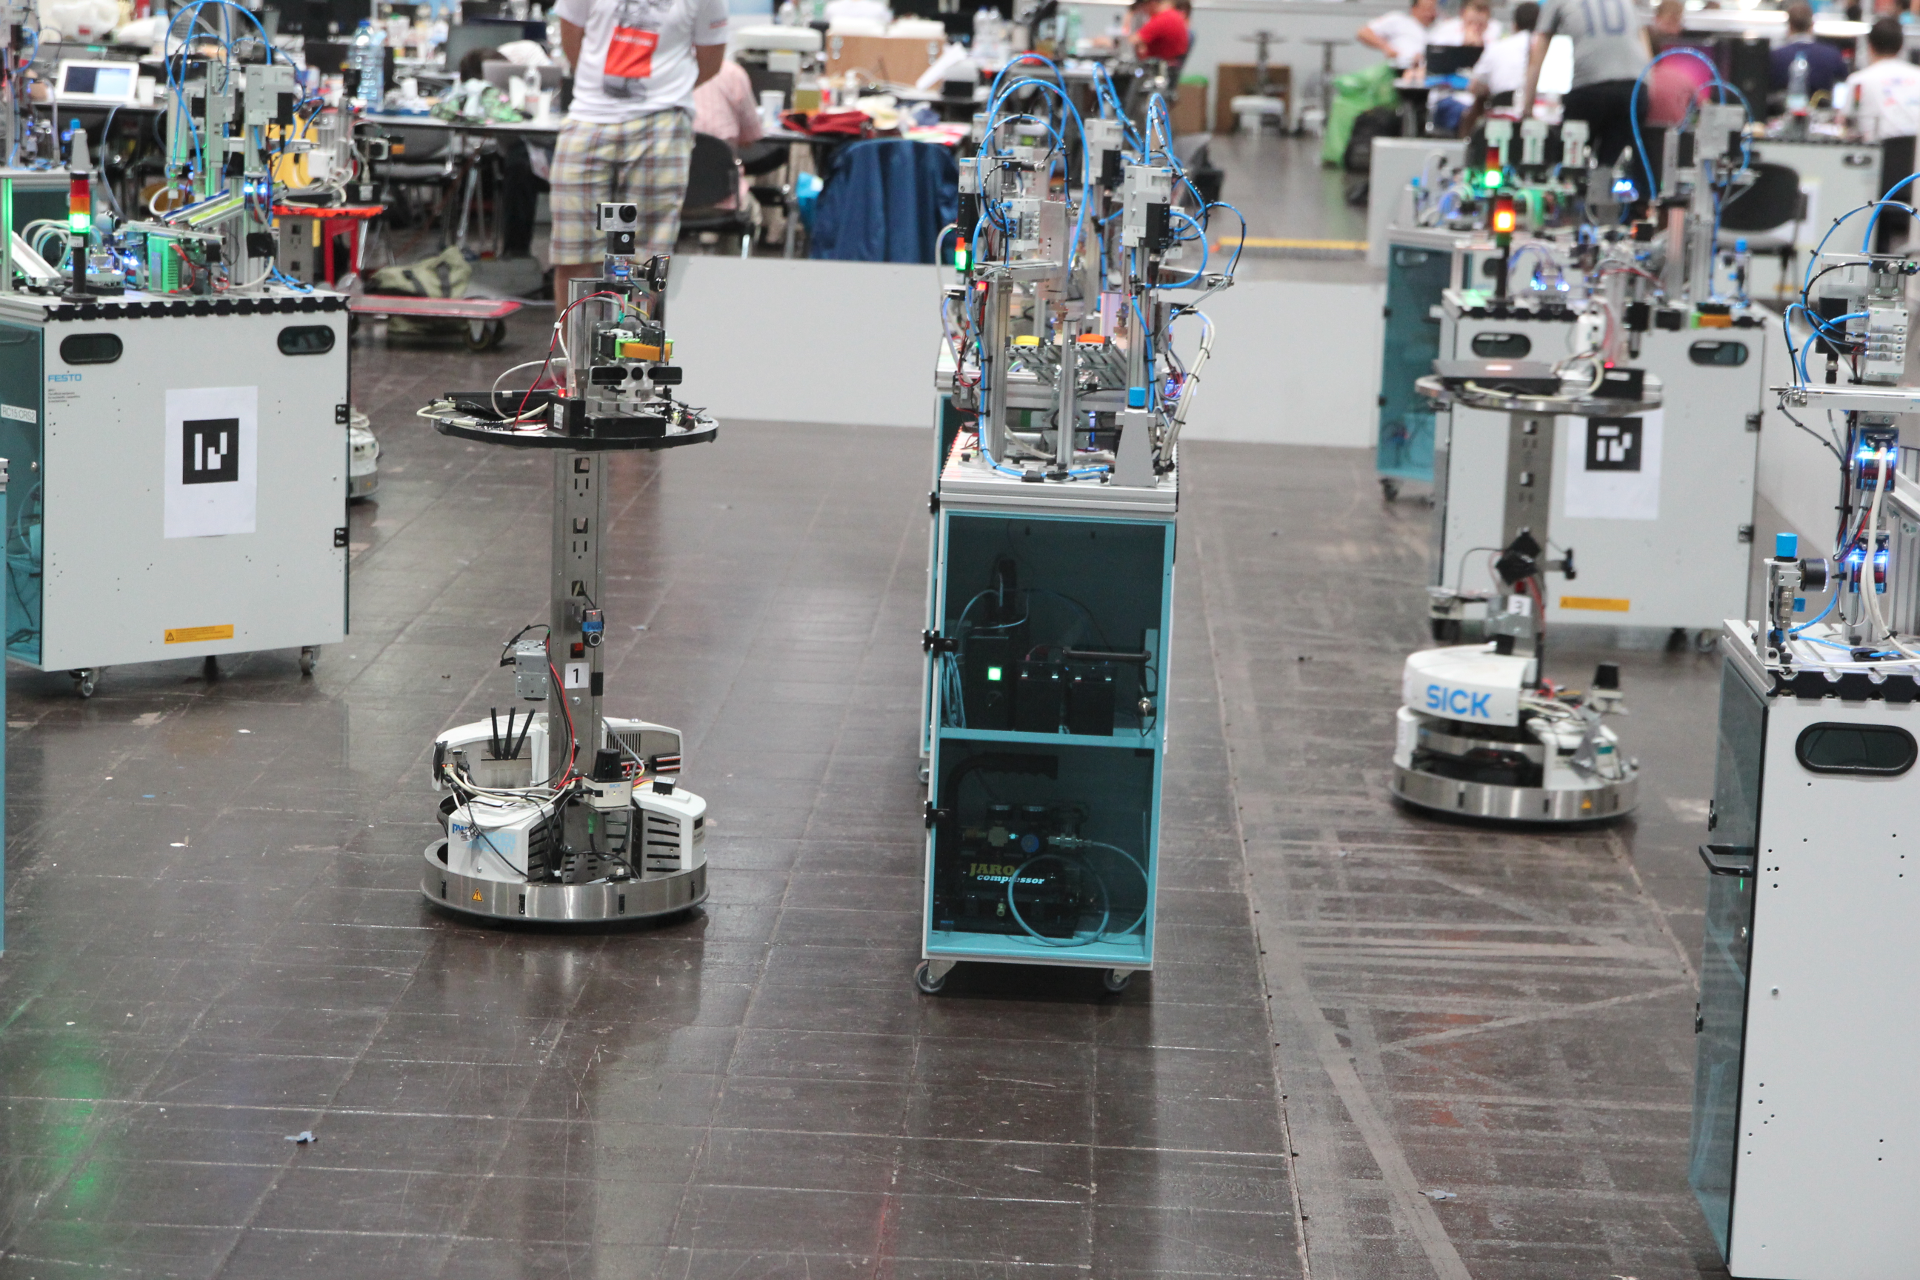
\includegraphics[width=0.5\textwidth]{../img/rcll-feld}
    \end{flushleft}
  \begin{description}[]
  \item[RoboCup Logistics League] \hfill \\
    \begin{itemize}
    \item Production logistics\\ in smart factory
    \item[$\Rightarrow$] Share world model
    \begin{itemize}
    \item[$\rightarrow$] between robots
    \item[$\rightarrow$] between global planner and reasoner executive
    \end{itemize}
    \end{itemize}
  \end{description}
    \end{column}
    \begin{column}{0.5\textwidth}
    \pause
    \begin{flushright}
    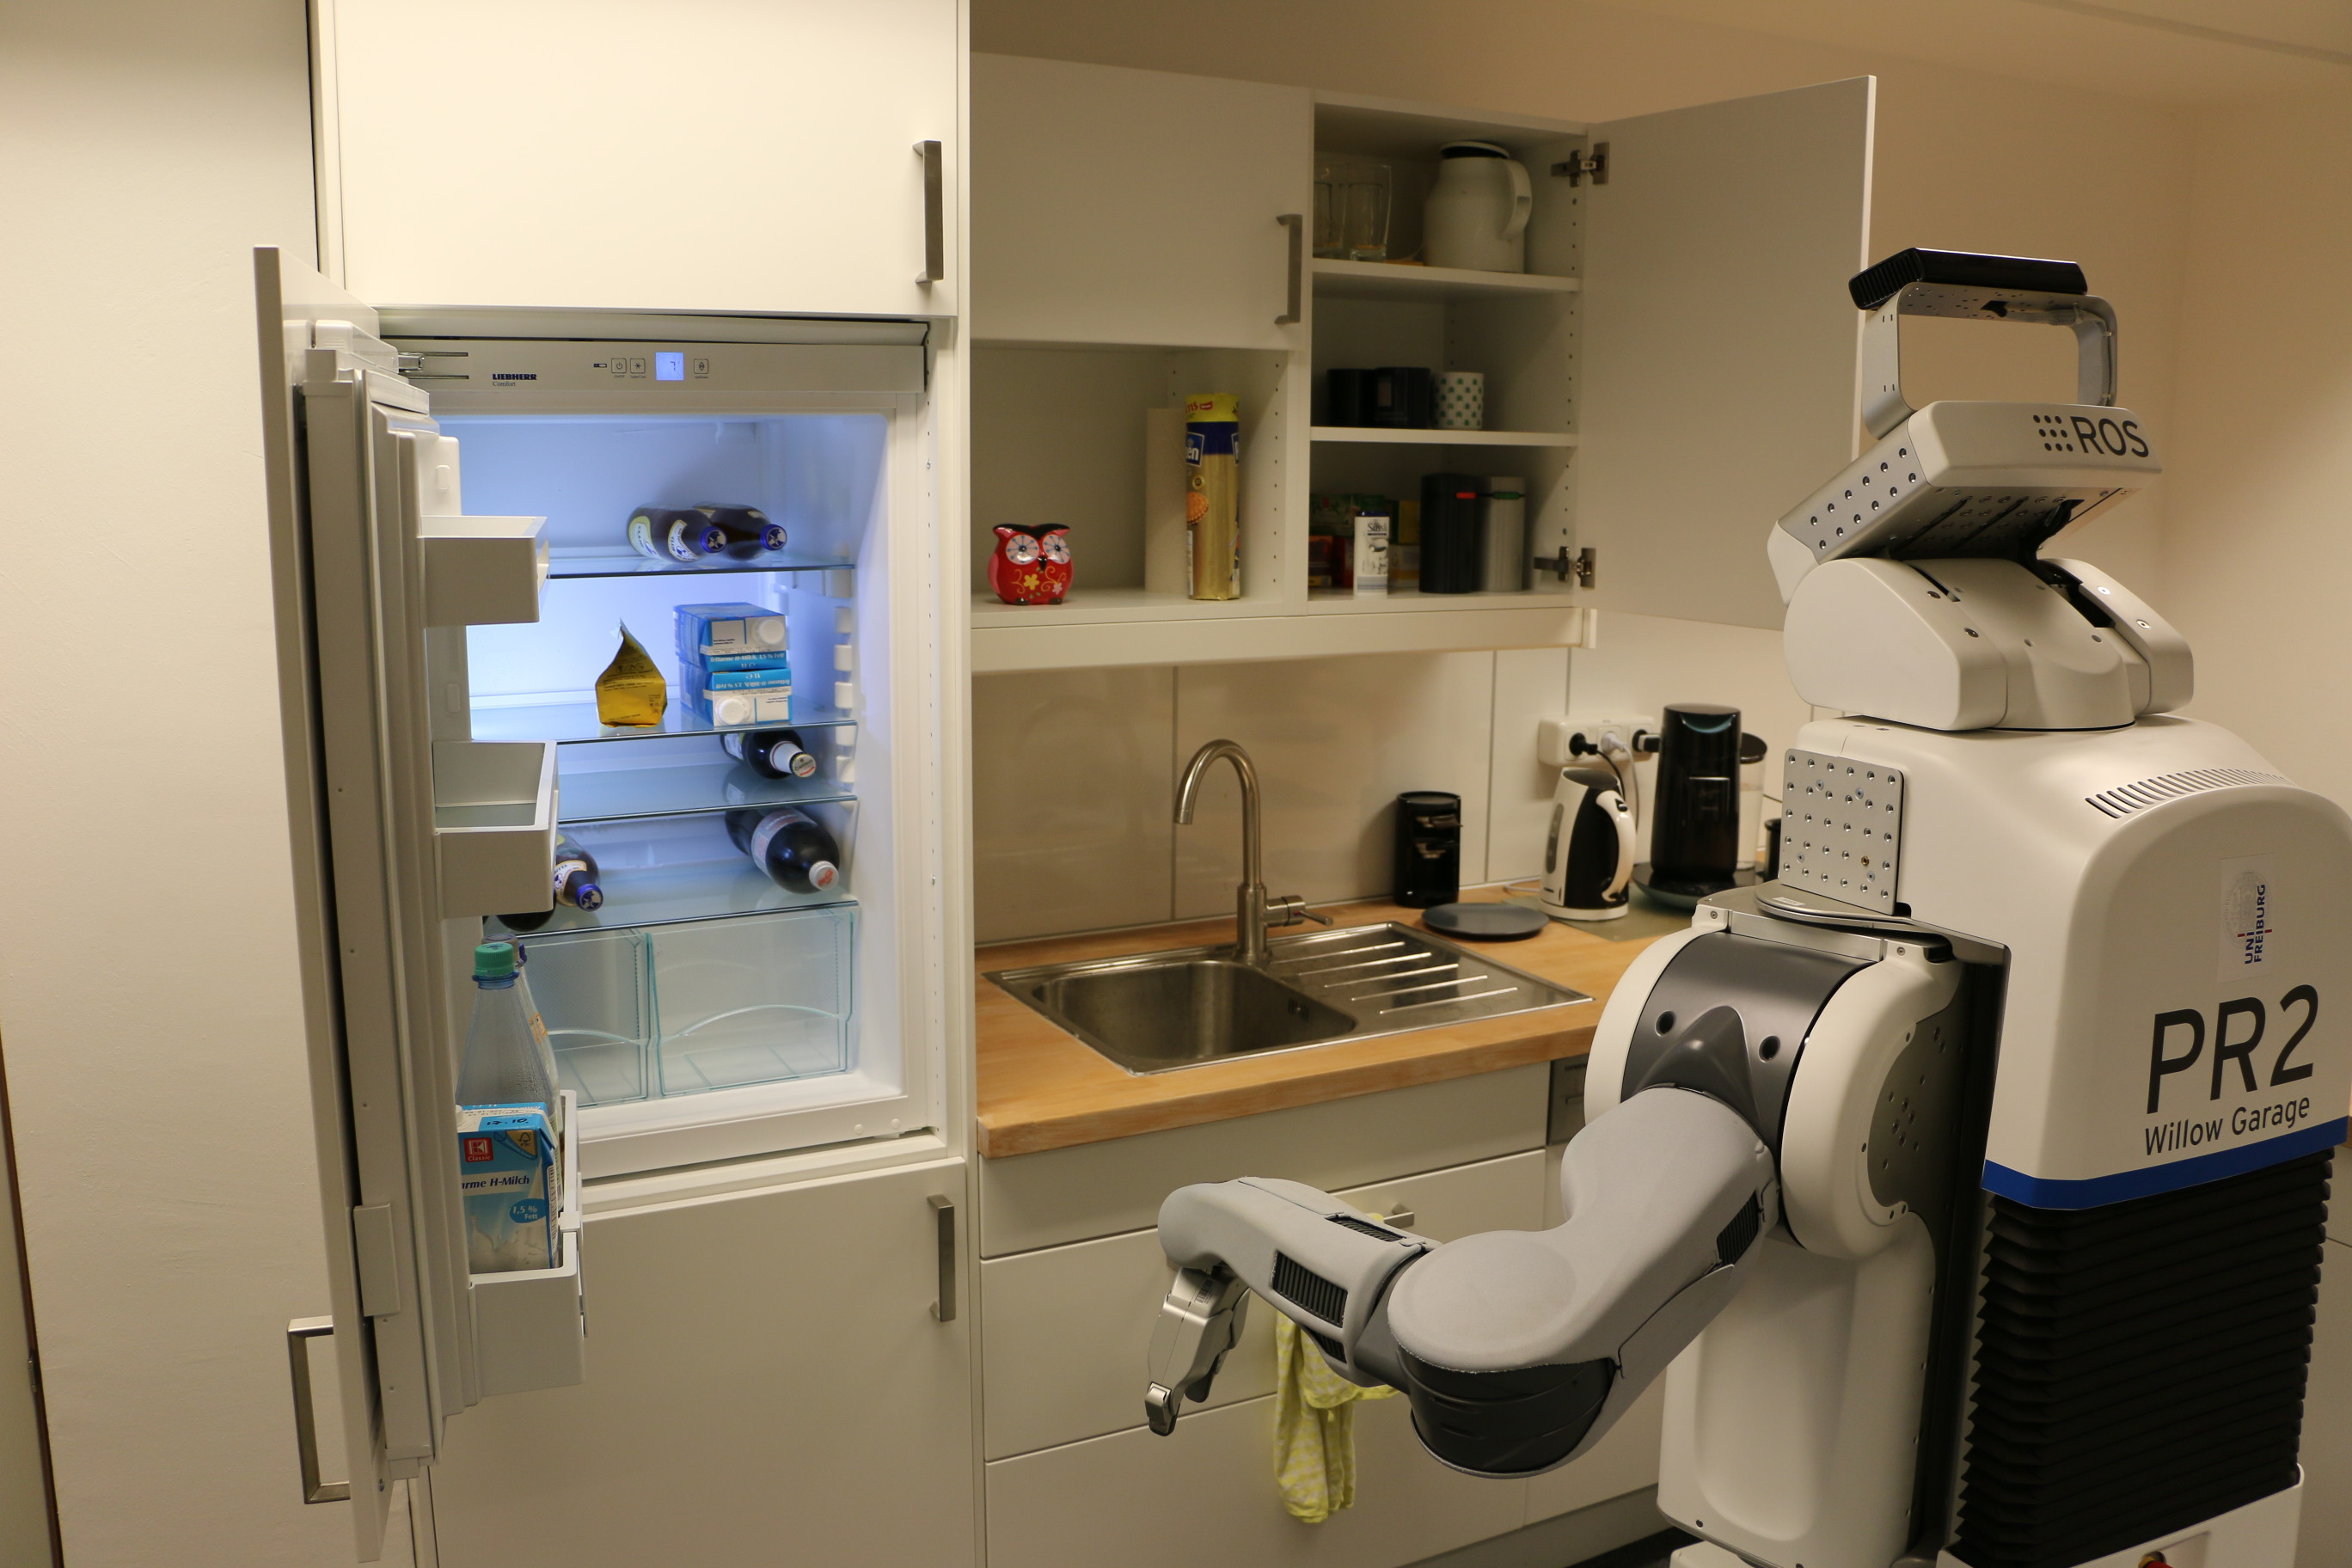
\includegraphics[width=0.5\textwidth]{../img/pr2-kbsg-kitchen}
    \end{flushright}
  \begin{description}[]
  \item[RoboCup@Home] \hfill \\
    \begin{itemize}
    \item Domestic service robots
    \item[$\Rightarrow$] Collect knowledge about concrete environment
    \item[$\Rightarrow$] Hybrid reasoning with spatio-temporal knowledge
    \item[$\Rightarrow$] Persistent storage
    \end{itemize}
  \end{description}    
    \end{column}
  \end{columns}
  
\end{frame}

\begin{frame}
  \frametitle{Background: Planners and Reasoners}
  \begin{columns}
  \begin{column}{0.83\linewidth}
  \begin{description}[]
  \item[CLIPS Rules Engine] \hfill \\
  \begin{itemize}
  \item First-Order Logic forward chaining systems
  \item Fact base and condition-action rules
  \item[$\Rightarrow$] Good for world model reasoning and\\ execution monitoring
  \end{itemize}
  \item[Planning Domain Definition Language]<uncover@2-> \hfill \\
  \begin{itemize}
  \item Standardized language for planning problems
  \item Domain description and problem description
  \item[$\Rightarrow$] Good for finding global plans
  \end{itemize}
  \item[Motion Planners]<uncover@3-> \hfill \\
  \begin{itemize}
  \item Robot arm, locomotion collision avoidance
  \item Depend on spatio-temporal data
  \item[$\Rightarrow$] Good for motion planning
  \end{itemize}
  \end{description}
  \end{column}
  \begin{column}{0.17\linewidth}
  
\includegraphics[width=\textwidth]{../img/CLIPS}
  \vspace{3.4cm}
  \pause\pause
  
\includegraphics[width=\textwidth]{../img/openrave}
  \end{column}
  \end{columns}
\end{frame}

\begin{frame}
  \frametitle{Background: Fawkes}
  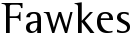
\includegraphics[width=0.2\textwidth]{../img/fawkes}  
  \begin{itemize}
    \item Robot Software Framework
    \item Component-based software design
    \item Blackboard communication infrastructure\\ with specific interfaces
    \item[$\Rightarrow$] Has no generic memory for knowledge sharing
  \end{itemize}
\end{frame}

\begin{frame}[fragile]
  \frametitle{Background: MongoDB}
  
\includegraphics[width=0.3\textwidth]{../img/mongodb}
  \begin{itemize}
    \item Document-oriented database
    \item Scalable, powerful and widely used
    \item Generic, schema-less data structure with key-value pairs
  \end{itemize}
\begin{columns}
\column[]{0.55\textwidth}
\begin{lstlisting}[style=ReallySmallJSON,
  framexleftmargin=2pt, xleftmargin=2pt,
 morekeywords={}, numbers=none]
 {
   type: "position",
   name: "robot1",
   translation: {x:2.5, y:1.0, z:0.0},
   rotation: {x:0.0, y:0.0, z:0.0, w:1.0},
   timestamp : ISODate("2016-05-19T15:26:34")
 }
\end{lstlisting}
\column[]{0.5\textwidth}
\begin{lstlisting}[style=ReallySmallJSON,
  framexleftmargin=2pt, xleftmargin=10pt,
 morekeywords={}, numbers=none]
db.positions.find(
  {
    type: "position",
    name: "robot1",
    timestamp : {"$gt":
      ISODate("2016-05-19T15:26:34")}
  })
\end{lstlisting}
\end{columns}
\pause
  \begin{itemize}
    \item Distributable with Replica Sets
    \item Expressive querying with JavaScript, MapReduce
    \item[$\Rightarrow$] Allows generic, scalable robot memory
  \end{itemize}
\end{frame}


\section{Approach}
\subsection{Goals}

\begin{frame}
  \frametitle{Goals}
\begin{description}[]
  \item[What should the robot memory be capable of?] \hfill \\
  \begin{itemize}
    \item Generic Storage and Retrieval
    \item Knowledge Sharing Between Knowledge Based Systems
    %% \item Special Views for Different Components
    \item Knowledge Computation on Demand
    \item Shared Knowledge for Multi-Robot Systems
    %% \item Spatio-Temporal Grounding
    \item Event Triggers
    \item Persistent Storage
    %% \item Human Interface and Visualization
  \end{itemize}
  \end{description}
\end{frame}

\subsection{Theoretical Foundation}
\begin{frame}
  \frametitle{Theoretical Foundation}
\begin{description}[]
  \item[Definition of documents representing knowledge] \hfill \\
  \small e.g.~$\{("object","cup"),("room","kitchen"),("position",{\scriptstyle\{("x",8),("y",4)\}})\}$
  \pause
  \begin{enumerate}
\item \textbf{Keys:} $\mathcal{K} := \Sigma^*$
\item  \textbf{Atomic values:} $\mathcal{V}_0$ are constants
\item \textbf{Unnested key-value pairs:} $\mathcal{P}_0:=\mathcal{K}\times\mathcal{V}_0$
\item \textbf{Unnested documents:} \vspace{-0.3cm}
%are sets of key-value pairs with unique keys and thus included in the power set of $\mathcal{P}_0$:\\
\begin{align*}
\mathcal{D}_0:=\{
  d\in\mathbb{P}(\mathcal{P}_0)|
  \forall (k,v),(k',v')\in d , k\neq k' \vee (k,v)=(k',v')
  \}
\end{align*}
\end{enumerate}
  \item[With nesting] \hfill \\
  \begin{enumerate}
\item  \textbf{Values:} $\mathcal{V}_n := \mathcal{V}_{n-1} \cup \mathcal{D}_{n-1}$
\item \textbf{Key-Value Pairs:} $\mathcal{P}_n:=\mathcal{K}\times\mathcal{V}_n$
\item \textbf{Documents:} \vspace{-0.3cm}
\begin{align*}
  \mathcal{D}_n:=\{
  d\in\mathbb{P}(\mathcal{P}_n)|
  \forall (k,v),(k',v')\in d , k\neq k' \vee (k,v)=(k',v')
  \}
\end{align*}
\end{enumerate}
  \end{description}
  \pause
  \textbf{Boundedly nested documents:} $\mathcal{D}=\cup_{n\in\{1..b\}}\mathcal{D}_n$\\
  \textbf{Values:} $\mathcal{V}=\cup_{n\in\{1..b\}}\mathcal{V}_n$, with nesting bound $b$
\end{frame}

\begin{frame}
  \frametitle{Theoretical Foundation}
  \begin{description}[]
  \item[Definition Robot Memory] \hfill \\
    \begin{enumerate}
      \item \textbf{Database:} finite set $\mathcal{DB} \subset \mathcal{D}$
      \item \textbf{Query:} represented by document $q\in\mathcal{D}$\\
      yields set of documents $r\subset\mathcal{DB}$ as result\\
      e.g. $q=\{("object","cup"),("room","kitchen")\}$
      \item \textbf{Computable:} $f: \mathcal{D} \rightarrow \mathbb{P}(\mathcal{D})$
      % providing computable knowledge on demand
      %computability and termination ensured by providing component
      \item \textbf{Set of Computables:} $\mathcal{C}$
      \item \textbf{Robot Memory:} $\mathcal{RM}=(\mathcal{DB},\mathcal{C})$
      \item \textbf{Memorized Documents:} $mem(\mathcal{RM})=DB \cup \bigcup_{f\in\mathcal{C}}f(\mathcal{D})$
    \end{enumerate}
  \end{description}  
\end{frame}

\begin{frame}
  \frametitle{Theoretical Foundation}
    \begin{description}[]
  \item[Mapping into PDDL] \hfill \\
\vspace{-0.5cm}
\small\begin{align*}
\text{e.g. } map_p&(\{("predicate", "at"),("object", "cup"),("room","kitchen")\})\\
             &= at(map_f("cup"), map_f("kitchen")) = at(cup, kitchen) \text{.}
\end{align*}
\pause
  \begin{enumerate}
      \item \textbf{Predicate symbols} $\mathcal{R}$, \textbf{Function symbols} $\mathcal{F}$
      \item \textbf{Name mapping:}
      \begin{align*}
        name_{pred}: \mathcal{R} \rightarrow \Sigma^* &\text{ and } name_{func}: \mathcal{F} \rightarrow \Sigma^*\\
        %injective, disjunct
        name_{pred-atr}: \mathcal{F} \times \mathbb{N} \rightarrow \mathcal{K} &\text{ and } name_{func-atr}: \mathcal{R} \times \mathbb{N} \rightarrow
\mathcal{K}
      \end{align*}
      \only<1-2>{
      \item \textbf{Map to function term:}
      \begin{align*}
        map_f(v)= &\text{ }v, v \in \mathcal{V} \setminus \mathcal{D}\\
        map_f(d)= &\text{ }f(map_f(v_1), ..., map_f(v_n)), \text{ iff } f \text{ is a n-array function in } \mathcal{F},\\
  ("functio&n", name_{func}(f))\in d, \forall i \in \{1..n\} (name_{func-atr}(f,i), v_i)\in d\\
  map_f(d)= &\text{ } nil_f, otherwise
      \end{align*}}
      \only<3>{
      \item \textbf{Map to function term}
      \item \textbf{Map to predicate:}
      \begin{align*}
        map_p(d)=&\text{ }p(map_f(v_1), ..., map_f(v_n)), \text{ iff } p \text{ is a n-array predicate in } \mathcal{R},\\
  ("predica&te", name_{pred}(p))\in d, \forall i \in \{1..n\} (name_{pred-atr}(p,i), v_i)\in d\\
  map_p(d)=& \text{ }nil_p, otherwise
      \end{align*}}
    \end{enumerate}
  \end{description}
\end{frame}

\subsection{Architecture}
\begin{frame}
  \frametitle{Architecture}
  \center
  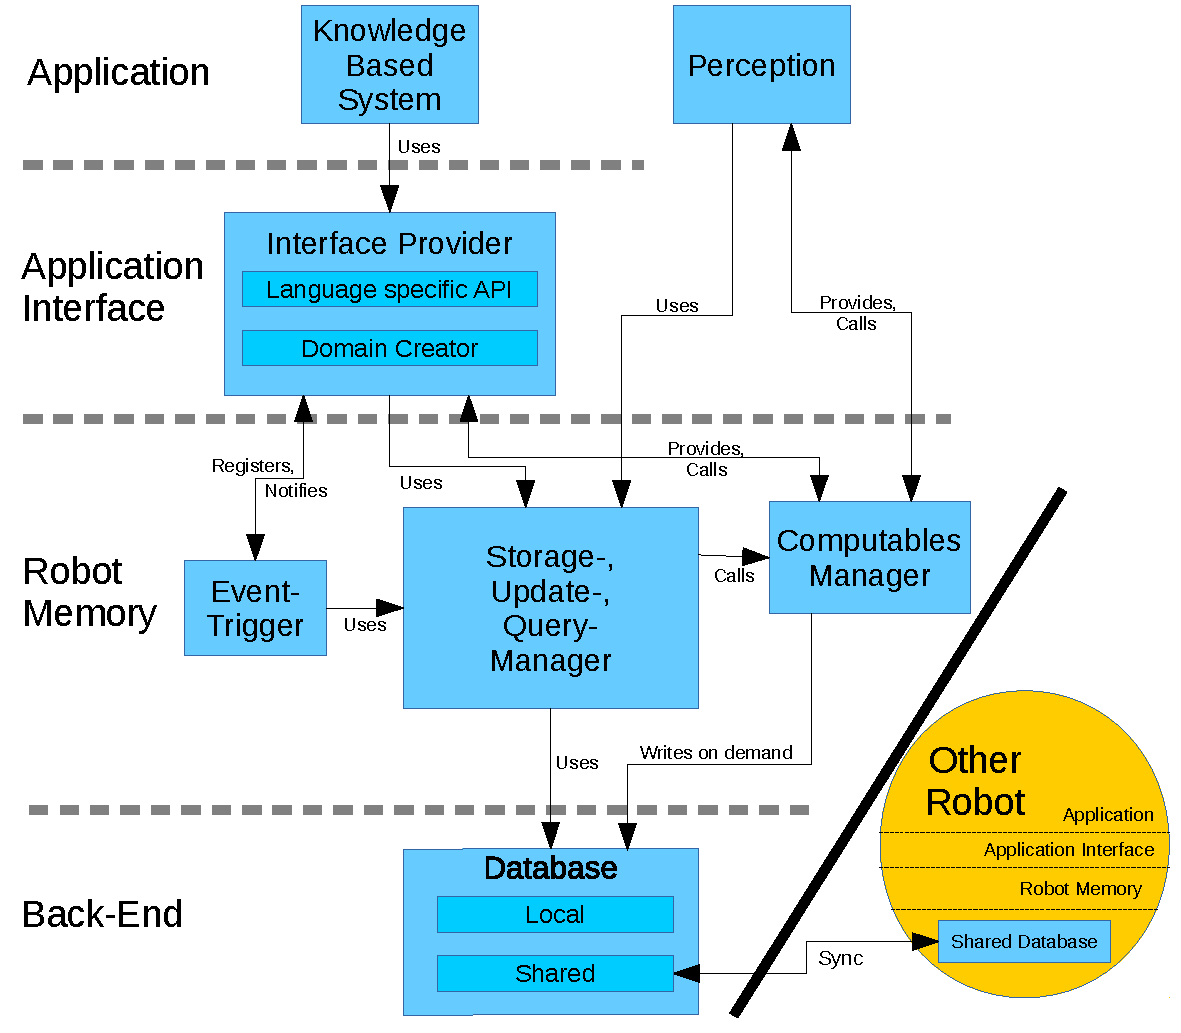
\includegraphics[width=0.8\textwidth]{../architecture.pdf}
\end{frame}

\subsection{Implementation}
\begin{frame}
  \frametitle{Implementation}
  \begin{description}[]
  \item[Back-End] \hfill \\
    \begin{itemize}
    \item Realized with MongoDB
    \item Replication for multi-robot distribution
    \end{itemize}
  \smallskip
  \pause
  \item[Robot Memory] \hfill \\
    \begin{itemize}
    \item Query enhancing, adding meta information (e.g. decay time)
    \item Dispatching raw DB queries and queries for computables
    \item Computables: forward query $\rightarrow$ compute results $\rightarrow$ \\
          cache results in DB $\rightarrow$ execute query on results
    \item Event-trigger with MongoDB Oplog
    \end{itemize}
  \smallskip
  \pause
  \item[Planner/Reasoner] \hfill \\
    \begin{itemize}
    \item Provide interface to robot memory\\
          (store/query features in CLIPS, domain creator in PDDL)
    \end{itemize}
  \end{description}  
\end{frame}

\section{Evaluation}
\begin{frame}
  \frametitle{Evaluation}
  %qualitative and quantitative
  \begin{tabular}{l|l}
  \textcolor{FawkesOrange}{\textbf{Prototype}} & \textcolor{FawkesOrange}{\textbf{Evaluation}}\\
  \hline
  \tabitem RCLL CLIPS agent & \tabitem Representing and querying\\
  ~~~~with world model sync & \tabitem Reasoner integration\\
                            & \tabitem Network throughput\\
                                 %% & \tabitem Event-trigger\\
  \hline
  \tabitem RCLL PDDL            & \tabitem Planner integration\\
  ~~~      domain creation      & \tabitem Knowledge Sharing\\
                                & ~~~~Planner-Reasoner\\
  \hline
  \tabitem @Home Computables & \tabitem Knowledge Sharing\\
  ~~~~                       & ~~~~Reasoner-Motion Planner\\
                             & \tabitem Hybrid Reasoning\\
  \hline
  \tabitem @Home Tidy up scenario & \tabitem Scalability\\
                                  & \tabitem Expressiveness vs.\\
                                  & ~~~~Computation Speed\\
\end{tabular}
\end{frame}

\section{Conclusion}
\begin{frame}
  \frametitle{Conclusion and Questions}

  \begin{block}{} \centering\bfseries The generic robot memory is capable of
    efficiently storing arbitrary symbolic or geometric information
    and allows consistent knowledge sharing and hybrid reasoning.
  \end{block}

  \bigskip

  \begin{itemize}
  \item Document-oriented representation and querying
  \item Theoretical and architectural design
  \item Interfaces for knowledge based systems
  \item Computables for on demand knowledge computation
  %% \item Implementation with MongoDB in Fawkes
  \item RCLL and @Home as application and evaluation domains
  \item Foundation for future projects
  \end{itemize}
\end{frame}

\end{document}
